\documentclass[a4paper]{article}
\usepackage{listings}
\usepackage{color}
\usepackage{fullpage}
\usepackage[htt]{hyphenat}
\usepackage{graphicx}


\definecolor{mygreen}{rgb}{0,0.6,0}
\definecolor{mygray}{rgb}{0.5,0.5,0.5}
\definecolor{mymauve}{rgb}{0.58,0,0.82}


\lstset{ %
  backgroundcolor=\color{white},   % choose the background color
  basicstyle=\ttfamily,        % size of fonts used for the code
  breaklines=true,                 % automatic line breaking only at whitespace
  captionpos=b,                    % sets the caption-position to bottom
  commentstyle=\color{mygreen},    % comment style
  escapeinside={\%*}{*)},          % if you want to add LaTeX within your code
  keywordstyle=\color{blue},       % keyword style
  stringstyle=\color{mymauve},     % string literal style
}



\author{\large Maria Ludovica Costagliola \\
        \small \textit{costagliola.1657716@studenti.uniroma1.it} \medskip\\
        \large Emanuele De Santis \\
        \small \textit{desantis.1664777@studenti.uniroma1.it}}
\title{Fibers implementation report\\
        \smallskip
        \small Advanced Operating Systems and Virtualization, A.A 2017/2018}
\date{}

\begin{document}

\maketitle
\section{Introduction}
This essay discusses the implementation of Fibers, made as final project for the \textit{Advanced Operating Systems and Virtualization} course. Fibers correspond to User-Level Threads and in Windows OS they are implemented at kernel-level. Through this project, we took care of inserting this functionality inside the Linux kernel. To accomplish it, we have developed a kernel module that implements all functionalities needed to support their execution.\bigskip\\
A Fiber can be seen as a lightweight thread of execution. Unlike usual kernel-level threads, Fibers have to explicitly yield the execution to let another fiber run.

\subsection*{\textit{MODULE}}
When the module is loaded, it will register the device that is needed to let the paradigm of IOCTL work, through \texttt{register\_fiber\_device()}, and several kprobes to have a sound and complete implementation of Fibers.\bigskip\\
At the unloading of the module, there is a cleanup function that takes care of unregistering all kprobes and removing the device file used for IOCTL.

\section{Kernel Level}
We developed the whole logic of Fibers at kernel level and made accessible to user-level the minimal amount of information possible.

\subsection*{\textit{DATA STRUCTURES}}
We used three main data structures to handle Fibers and related information:
\begin{itemize}
  \item \texttt{struct process}
  \item \texttt{struct thread}
  \item \texttt{struct fiber}
\end{itemize}
The \texttt{struct process} is unique inside the process and is initialized by the first thread of the process that converts to a fiber: we register here the number of active threads of the process, the number of fibers created until that point, two hashtables to keep trace of all converted threads and of all fibers created by whatever thread of the process. There are also the \texttt{process\_id} and a \texttt{struct hlist\_node}, both needed to insert this process inside a global hashtable that contains all active processes that are using Fibers.\bigskip\\

\lstinputlisting[language=C, firstline=78, lastline=85]{../module/fibers.h}\bigskip
Each thread that wants to convert to a fiber will initialize a \texttt{struct thread} that contains \texttt{thread\_id} and a \texttt{struct hlist\_node} to be inserted in the hashtable of the parent process; there is a pointer to the \texttt{struct process} of its parent process and a pointer to the fiber that it is currently running.\bigskip\\

\lstinputlisting[language=C, firstline=87, lastline=92]{../module/fibers.h}\bigskip
Finally, the fundamental data structure is the \texttt{struct fiber}, one for each fiber. In this struct there is a lock used to serialize threads requests to switch to that fiber. There is also a pointer to the parent process and the thread executing this fiber. The struct contains a \texttt{struct pt\_regs} and \texttt{struct fpu} to be able to save and restore its execution context. In the struct there are also starting address of the fiber's stack and its size. To handle FLS (\textit{Fiber Local Storage}), there is an array of fixed size \texttt{MAX\_FLS\_POINTERS}, and a bitmap to quickly find available cells inside the array. The last fields in this data structure are needed to compute some statistics to be shown inside proc subsystem.\bigskip\\

\lstinputlisting[language=C, firstline=45, lastline=75]{../module/fibers.h}

\subsection*{\textit{IOCTL}}
The file \texttt{ioctl.c} comes into play each time is issued an IOCTL call at user level. We have seven IOCTL commands, one for each functionality the module has to handle, that are defined inside \texttt{ioctl.h} and are associated to a different number, from 0 to 6.\bigskip\\
The registered function is \texttt{fibers\_ioctl()}. It checks the IOCTL command issued and calls the appropriate function to perform the desidered task. If the user was supposed to pass some parameters (wrapped in a \texttt{struct fiber\_arguments}), there is a check on this structure (to verify that the address passed is a valid one) and then it is copied inside a local structure. At the end, we call the actual function that performs the task requested by the user.\bigskip\\
In case of a switch, we pay attention to take a lock right before calling the actual switch function and release it as soon as this function returns. This mechanism is used since we are in an SMP context to be safe and secured.\bigskip\\
If the user issues an IOCTL call to get a value inside the fiber local storage, then it is important to make a \texttt{copy\_to\_user} with this just retrieved value, since the user-level stub for IOCTL returns an int (to maintain compatibility with the old signature of IOCTL handler).\bigskip\\
The actual functions are implemented inside \texttt{fibers.c}.

\subsection*{\textit{CONVERT A THREAD TO A FIBER}}
In order to use Fibers' logic, it's important to have a first fiber to start with. The function \texttt{do\_ConvertThreadToFiber} is called by each thread that wants to use Fibers for the first time. The very first thread in a process that calls it, has to initialize the \texttt{struct process} data structure related to the process the thread lives in.\bigskip\\
\texttt{do\_ConvertThreadToFiber} has to create the \texttt{struct process} only if it doesn't yet exists. To do so in a SMP context it uses a lock.\bigskip\\
After that, it creates also a \texttt{struct thread} representing the thread and a \texttt{struct fiber} representing the first fiber for that thread.
This $special$ fiber uses the current value of the \texttt{rip} register as starting point and is automatically marked as running by that thread.\bigskip\\
This function returns the id of the newly created fiber.

\subsection*{\textit{CREATE A NEW FIBER}}
Using this funtionality, a thread has the possibility to create a new fiber, assigning to that a starting address (usually a function pointer) and a parameter to be passed.\bigskip\\
In our module this functionality is implemented through \texttt{do\_CreateFiber}. This function looks for the process and the thread in the respective hashtables (if it doesn't find even one of them, it means that the calling thread has not perfomed the \texttt{ConvertThreadToFiber} call yet).\bigskip\\
After these checks, it allocates a new \texttt{struct fiber}, computes the stack pointer using the base stack address and the stack size and adds the struct to the process's hashtable.\bigskip\\
It then returns the id of the newly created fiber.

\subsection*{\textit{SWITCH TO A FIBER}}
Since Fibers are not preemptable, they have to yield the execution to let another fiber run. To do so our module uses the \texttt{do\_SwitchToFiber} function.\bigskip\\
This function first checks if the selected fiber is not running (in fact if it is already running it has to fail) and cares to save the CPU and FPU status in the \texttt{struct fiber} related to the previous fiber and to restore the CPU and FPU context taken form the next \texttt{struct fiber}.\bigskip\\
It has also to reflect the switch in the control pointers both of the \texttt{struct thread} and of the \texttt{struct fiber}.

\subsection*{\textit{FIBER LOCAL STORAGE}}
Each fiber shares the address space with each other fiber and each other normal kernel thread. To let a fiber have its own local space, we implement a Fiber Local Storage as an array of \texttt{long long} of fixed size. There are 4 APIs to interact with this local storage:

\begin{itemize}
  \item \texttt{do\_FlsAlloc}
  \item \texttt{do\_FlsSetValue}
  \item \texttt{do\_FlsGetValue}
  \item \texttt{do\_FlsFree}
\end{itemize}\bigskip
In this way, each fiber can allocate a cell, set a value for that cell, read that value and free the cell.
To better perform these operations we have used a bitmap: in this way we can find a free space in $O(\log n)$ instead of $O(n)$.\bigskip\\
Each function checks the validity of the arguments passed to be always safe.

\subsection*{\textit{KPROBES}}
Our module needs a kprobe to release all the memory used once a thread or the whole process die. This kprobe is executed each time \texttt{do\_exit()} is called. Since \texttt{do\_exit()} is called when the current thread is about to die, this is the right place to free all our structures regarding that thread. Moreover, if the current thread is the last one in the process still executing fibers, this leads to a complete cleanup of all \texttt{struct fiber} belonging to that process and the \texttt{struct process} itself.\bigskip\\
We also rely on kprobes to patch the \texttt{/proc/\{PID\}} directory to show up also the \texttt{fibers} folder only in those processes that have at least one fiber.\bigskip\\
We use a third kprobe to update fiber's execution time whenever the system schedule runs.

\subsection*{\textit{PROC SUBSYSTEM}}
Each fiber stores some information needed to compute runtime statistics about its usage. These statistics are displayed in a pseudofile named with the fiber id in \texttt{/proc/\{PID\}/fibers}.\bigskip\\
\texttt{/proc/\{PID\}} has a very particular structure, different with respect to a normal proc directory/file. In fact, all elements appearing in \texttt{/proc/\{PID\}} are defined in a static constant array (in \texttt{/fs/proc/base.c}) named \texttt{tgid\_base\_stuff}.
To add the folder \texttt{fibers} to \texttt{/proc/\{PID\}}, we had to modify the behaviour of the \texttt{iterate\_shared} handler (in this case \texttt{proc\_tgid\_base\_readdir}) and the \texttt{lookup} handler (in this case \texttt{proc\_tgid\_base\_lookup}). We did it using two kretprobes.\bigskip\\
We examine the case of the \texttt{iterate\_shared} since the other one uses almost the same approach. In this case we compute once (as soon as the kretprobe is fired for the first time) the number of entries added by the actual \texttt{proc\_pident\_readdir}, called by \texttt{proc\_tgid\_base\_readdir}, and then we call again \texttt{proc\_pident\_readdir} to insert an ad-hoc array containing only the \texttt{fibers} entry. In this way the inode for our entry is instantiated exactly like the ones corresponding to the actual entries of \texttt{tgid\_base\_stuff} and the \texttt{dir\_context} is update accordingly.\bigskip\\
To show under \texttt{/proc/\{PID\}/fibers} all the pseudofiles corresponding to the fiber instantiated in that process, we used the same approach of \texttt{tgid\_base\_stuff} and \texttt{proc\_pident\_readdir}, but this time the array is not a static constant array, but it is dynamically generated based on the fibers present in the process.\bigskip\\
Each of these files has the same \texttt{read} handler, that extract information from its argument \texttt{struct file}, to understand which fiber's information outputs to user-level.

\section{User Level}
To make visible to user-level applications all interfaces we did in the kernel code, we developed an user-level library that is able to take the user-level application's call and redirect in the correct way to the kernel module using IOCTL.\bigskip\\
Since we use a dynamically assigned major number for the device \texttt{/dev/fibers} to compute IOCTL commands' numbers, we had to find a way to pass these numbers to user-space.
The solution was to implement a \texttt{read} handler for \texttt{/dev/fibers} (besides the \texttt{unlocked\_ioctl}) that outputs the IOCTL commands' numbers in a predefined scheme.\bigskip\\
The user-space library registers a constructor that opens a file descriptor to \texttt{/dev/fibers}, reads on it and stores the numbers, following the predefined scheme.\bigskip\\
Moreover it wraps all the IOCTL calls to hide the complexity to the user and to pass the data the user provides in the correct manner.

\section{Performances}
Using the given benchmark application, we was able to perform a basic performance test of our module with respect to the user-space implementation.
In the first case we run 15 iteration with a growing number of fibers (each time 32 fibers more than the previous time).
In the second case we run again 15 iteration of the test application with 550 fibers running and we collected the results.\\We used PyPlot to plot all the data collected.

\begin{center}
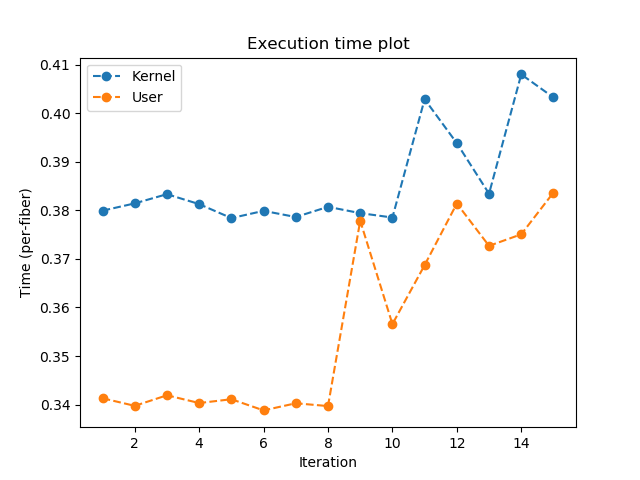
\includegraphics[scale=0.65]{../perf/user-kernel}\bigskip\\
\end{center}

As we can see in this first plot, it is clear that our module usually takes more time with respect to the user-space implementation. This is because of the context switches from user-space to kernel-space and vice versa. We can also notice a deterioration of the performances as the time goes on caused by CPU throttling (in fact the benchmark generates a lot of CPU work, so the CPU temperature increases).\\
Anyway, it is possible to see that kernel level implementation runs approximately in constant time with respect to the number of fibers (in fact the kernel module is called approximately $O(n)$ times and the per-fiber time remains almost the same).

\begin{center}
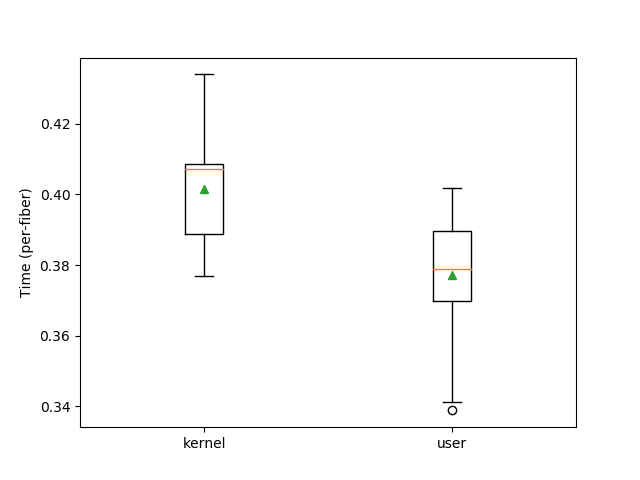
\includegraphics[scale=0.65]{../perf/boxplots}\bigskip\\
\end{center}

These boxplots show us a more compact view over all iterations both for kernel-space implementation and for user-space implementation fixing the number of fibers to 550.
It shows for each implementation the quantiles (black horizontal lines), the median (yellow horizontal line) and the mean (green triangle) given from the samples we took during the iterations.\\
From this view it possible to clearly see that, except for outliers, the majority of the kernel-implementation times are very close to the user-implementation times, so the median kernel overhead is very small.

\end{document}
